\chapter{Estad\'istica de datos orientados}
\label{ch:prob}

Antes de revisar el tema principal de este cap\'itulo es conveniente revisar algunos temas de probabilidad que son comunes o equivalentes.

\section{Variables aleatorias}
\label{s:randomVar}

Una variable aleatoria es una funci\'on en donde el dominio es un espacio de posibles opciones $S$ y la imagen son los n\'umeros reales $\mathbb{R}$ \citep{casella_statistical_2002}.
El t\'ermino \textit{aleatorio} en la definici\'on hace referencia a la ley probabilidad y no significa que tenga la misma probabilidad en cualquier intervalo de su imagen. A largo de este escrito se entender\'a de esta manera.

\textit{Notaci\'on}: Las variables aleatorias se denotar\'an con letras may\'usculas, $X$ por ejemplo. Por otro lado, las realizaciones/observaciones de esta variable aleatoria (o su imagen) ser\'an denotadas con las correspondientes letras min\'usculas, $x$ para el ejemplo anterior. A diferencia del cap\'itulo anterior en que $x$ y $X$ indicaban ubicaci\'on espacial, en este cap\'itulo y el que sigue se utilizar\'a para referirnos a una variable aleatoria.
%Como ejemplo m\'as espec\'ifico tenemos el siguiente: $X$, la estatura de los mexicanos, puede tomar el valor $x=1.7$ m.

El objeto de estudio de este proyecto doctoral fueron fen\'omenos que se modelaron con variables aleatorias continuas, es decir, variables aleatorias cuya imagen pod\'ia tomar cualquier valor dentro de cierto intervalo no nulo de los reales.

Las funciones aleatorias son completamente caracterizadas por su funci\'on de distribuci\'on de probabilidad $F$, tambi\'en conocidas como funci\'on de distribuci\'on acumulativa (CDF, por sus siglas en ingl\'es):

\begin{equation}
	F_X(x) = P_X(X \le x), \qquad \forall x. 
	\label{e:cdf1D}
\end{equation}

\noindent
donde $P$ denota la probabilidad de que la variable aleatoria $X$ sea menor o igual que el valor $x$.
%Por ejemplo, la probabilidad de que la estatura, $X$, sea menor que $x = 1.5$ m.

Para caracterizar completamente una variable aleatoria continua $X$, alternativamente a la funci\'on de distribuci\'on $F$, se tiene la funci\'on de densidad de probabilidad $f$:

\begin{equation}
	F_X(x) = \int_{-\infty}^x f_X(t)dt \qquad \forall x.
\end{equation}

Si $f_X(x)$ es continua, entonces, por el teorema fundamental del c\'alculo:

\begin{equation}
	\frac{d}{dx}F_X(x) = f_X(x)
\end{equation}

El histograma es un estimador de la funci\'on de densidad $f_X$.

Para mostrar las caracter\'isticas de una CDF usemos la diferencia hacia adelante de primer orden:

\begin{equation}
\label{e:ForwDiff} % "Forw"ard "Diff"erence
\Delta F :=F(x+d)-F(x)
\end{equation}

Una funci\'on de distribuci\'on $F$ satisface las siguientes condiciones:

\begin{itemize}
	\item $F(x)$ es una funci\'on no-decreciente de $x$. Es decir, $\Delta F \ge 0$.
	\item $F(x)$ continua por la derecha. Es decir, para cada n\'umero $x_0$, $\lim_{x \to x_0^+}F(x) = F(x_0)$.
	\item $\lim_{x \to -\infty}F(x) = 0$, y  $\lim_{x \to +\infty}F(x) = 1$.
\end{itemize}

N\'otese que no hay significado probabil\'istico en estas definiciones, dicha interpretaci\'on se obtiene a partir de la definici\'on en la \autoref{e:cdf1D}. Gr\'aficamente, todas estas caracter\'isticas se pueden observar en la \autoref{f:cdf1D}.

\begin{figure}
	\centering
	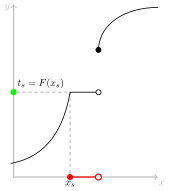
\includegraphics{distributionFunction}
        \caption{Ejemplo de funci\'on de distribuci\'on de probabilidad. En rojo se muestra la inversa $F^{-1}(t_s)$.}
	\label{f:cdf1D}
\end{figure}

Sea $S:= \{x_1, \ldots, x_n\}$ el conjunto formado por observaciones (valores medidos o muestreados) de la variable aleatoria $X$. Entonces se pueden estimar los valores de la funci\'on de distribuci\'on $F$ a partir de su funci\'on de distribuci\'on emp\'irica.

\begin{equation}
\label{e:empF} % "e"quation of the "Emp"irical Distribution function Fn.
\hat{F_n} (x) = \frac{1}{n}\sum_{k=1}^{n} \mathbbm{1} (x_k \le x)
\end{equation}

\noindent
donde $\mathbbm{1}$ es la funci\'on indicador (\autoref{e:indicatorFunc}) y $n$ es la cantidad de datos.

Esta funci\'on emp\'irica es la funci\'on no param\'etrica aproximante m\'as conocida de una funci\'on de distribuci\'on, pero tambi\'en existen otras como la de Weibull plotting position \'o est\'andar \citep[p. 10]{salvadori_extremes_2007}.
No se debe confundir con la unci\'on de densidad de Weibull, la cual es continua. En este trabajo utilizaremos la \autoref{e:empF} debido a su simplicidad y a su similitud con la c\'opula emp\'irica que se ver\'a m\'as adelante.

A partir de ahora, en lo que resta de esta subsecci\'on, supondremos que los datos observados $x_i$ est\'an ordenados en orden creciente ($x_i < x_{i+1}$) y no hay datos duplicados, es decir, que los datos son iguales a sus estad\'isticos de orden $x_{(i)}$.

El gr\'afico de la funci\'on de distribuci\'on emp\'irica (\autoref{f:empCDF}) es constante a tramos con saltos de magnitud $1/n$ cada $x_i$.
%En cada salto, los puntos rellenos representan un punto en la curva $\hat{F_n}$ mientras que los puntos vac\'ios representan un punto que \textit{no} pertenece a la funci\'on de distribuci\'on emp\'irica.
Si definimos las \textbf{pseudo-observaciones} como $u_i := \hat{F_n}(x_i)$,
%entonces los puntos rellenos tienen coordenadas $(x_i, u_i)$.
interpretada como una probabilidad en el intervalo $[0,1]$, $u_i$ es una cantidad adimensional.

\begin{figure}[H]
	\centering
	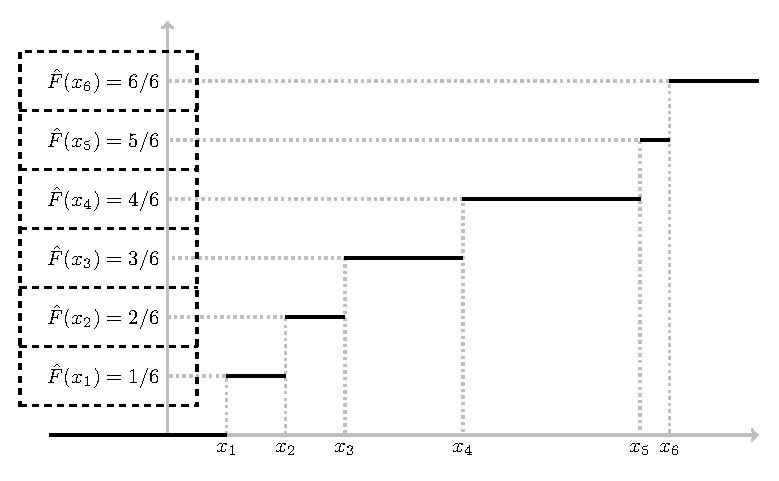
\includegraphics{empCDF}
	\caption{Funci\'on de distribuci\'on emp\'irica. Los rect\'angulos en negro con l\'ineas de guiones se muestra el correspondiente arreglo computacional para almacenar los valores de $\hat{F}_n$.}
	\label{f:empCDF}
\end{figure}

Desde el punto de vista computacional, para obtener valores de esta funci\'on emp\'irica solamente basta con almacenar los valores de $\hat{F}_n(x_i)$, para toda $i=1,\ldots, n$.

$$
\begin{array}{| c | c | c | c | c | c |}
	\hline
	\hat{F}_n(x_1) & \hat{F}_n(x_2) & \hat{F}_n(x_3) & \cdots & \hat{F}_n(x_{n-1}) & \hat{F}_n(x_n) \\ \hline
\end{array}
$$

De esta manera para saber el valor de $\hat{F}_n$ en cualquier otro valor $x$, solamente hay que compararlo contra todas las observaciones y saber cu\'al $x_i$ es el inmediato inferior.
Esto es lo que significa la \autoref{e:empF}: para obtener un valor $\hat{F}(x)$, $x$ se compara con cada observaci\'on $x_i$.
N\'otese que ya no se requieren los valores $x_i$ ya que est\'an impl\'icitos en vector de valores de $\hat{F}_n$, solamente es necesario saber cu\'al es el \'indice $i$ para poder acceder al arreglo.
Para lenguajes de programaci\'on de bajo nivel como C/C++ o Fortran, esto se pudiera implementar en un arreglo de enteros sin signo, lo que reduce el uso de memoria comparado con un arreglo de n\'umeros reales (valores flotantes).
Los \'indices de la \autoref{f:empCDF} corresponden uno-a-uno con arreglos de lenguajes de programaci\'on con offset $1$ como R o Matlab, pero no para arreglos de lenguajes programaci\'on de offset $0$ como Python o C++.
A\'un m\'as, pudiera ahorrarse guardar tal arreglo ya que el c\'alculo de $1/i$ es computacionalmente muy r\'apido.

La implementaci\'on computacional de la funci\'on de distribuci\'on emp\'irica est\'a en la funci\'on \verb|stats::ecdf| del software \verb|R|.

Como puede verse en la \autoref{f:empCDF}, la funci\'on de distribuci\'on emp\'irica no es continua, pero existen muchos modelos que s\'i lo son. Por ejemplo, se encuentran la funci\'on normal, la lognormal, ley de potencias, Weibull, exponencial, entre otras. Estos ejemplos, salvo la distribuci\'on normal, tienen asimetr\'ia positiva, y son com\'unmente utilizadas en el modelado de las longitudes de fracturas \citep{bonnet_scaling_2001,bour_connectivity_1997,gudmundsson_power-law_2011}. Aunque estas distribuciones dependen de ciertos par\'ametros (la media y la varianza en el caso de la distribuci\'on normal), tambi\'en existen funciones de distribuci\'on no param\'etricas. Otras variables que pueden ser modeladas con dichas funciones son la apertura, la porosidad y la permeabilidad.

En muchas ocasiones unos de los objetivos buscados mediante el an\'alisis y modelado de los datos es la simulaci\'on, ya que permite cuantificar la incertidumbre del fen\'omeno. Un algoritmo de simulaci\'on denominado de la transformada inversa requiere la funci\'on cuantil. \'Esta es una funci\'on asociada con una variable aleatoria $X$, la cual se define como la inversa generalizada $F^-:[0,1] \to \overline{\mathbb{R}}= [-\infty, \infty]$ de la funci\'on de distribuci\'on $F$ \citep{embrechts_note_2013}:

\begin{equation}
	F^-(y)= \inf \{x \in \mathbb{R}:F(x) \ge y\}
	\label{e:generalizedInv}
\end{equation}

\noindent
con la convenci\'on que $\inf \emptyset = \infty$. Esta inversa puede visualizarse en la \autoref{f:cdf1D}. Si $F$ es estrictamente creciente, entonces $F^- = F^{-1}$, la inversa generalizada es igual a la inversa usual.

Dicha funci\'on cuantil, puede o no existir en forma expl\'icita independientemente si la funci\'on $F$ existe en forma expl\'icita. Por ejemplo, se tiene una f\'ormula algebraica para la funci\'on de densidad de la distribuci\'on normal pero no se tiene una para calcular la funci\'on de distribuci\'on o la funci\'on cuantil, para estos casos se tiene que recurrir a m\'etodos num\'ericos. Un ejemplo parecido es el encontrado con la funci\'on de densidad de von Mises (V\'ease \autoref{ss:circularStats}).

Un ejemplo opuesto se tiene con los polinomios de Bernstein-Kantorovich \citep{munoz-perez_estimating_1987}, que representan de forma semi-expl\'icita la funci\'on cuantil, pero para obtener su correspondiente funci\'on de distribuci\'on se tiene que recurrir a m\'etodos num\'ericos \citep{quarteroni_numerical_2006,dahlquist_numerical_2008}. Esta funci\'on no param\'etrica y continua es un caso particular de una curva de B\'ezier (ver \autoref{ch:approxTheory}). La implementaci\'on computacional de esta funci\'on puede ser utilizada mediante la funci\'on \verb|lmomco::dat2bernqua| \citep{asquith_lmomco:_2017}.

Encontrar num\'ericamente la inversa de una funci\'on $F$ para un valor $y$ en su imagen, es equivalente a encontrar la ra\'iz $x$ de la funci\'on $G(x,y)= F(x) - y = 0$. Una implementaci\'on computacional para encontrar dicha ra\'iz se puede encontrar en el software R con la funci\'on \verb|stats::uniroot|. Otra funci\'on que podr\'ia ser m\'as r\'apida es utilizando una versi\'on paralelizada del m\'etodo de bisecci\'on para encontrar dicha ra\'iz \citep{miranker_survey_1971,nijmeijer_parallel_2015,stack_overflow_algorithm_2017,karniadakis_parallel_2003}. Tambi\'en se puede aprovechar el hecho de que la funci\'on $G$, debido a que es una traslaci\'on de $F$, es mon\'otona.


% \chapter{Estad\'istica de datos orientados}
\label{ch:prob}

Antes de revisar el tema principal de este cap\'itulo es conveniente revisar algunos temas de probabilidad que son comunes o equivalentes.

\section{Variables aleatorias}
\label{s:randomVar}

Una variable aleatoria es una funci\'on en donde el dominio es un espacio de posibles opciones $S$ y la imagen son los n\'umeros reales $\mathbb{R}$ \citep{casella_statistical_2002}.
El t\'ermino \textit{aleatorio} en la definici\'on hace referencia a la ley probabilidad y no significa que tenga la misma probabilidad en cualquier intervalo de su imagen. A largo de este escrito se entender\'a de esta manera.

\textit{Notaci\'on}: Las variables aleatorias se denotar\'an con letras may\'usculas, $X$ por ejemplo. Por otro lado, las realizaciones/observaciones de esta variable aleatoria (o su imagen) ser\'an denotadas con las correspondientes letras min\'usculas, $x$ para el ejemplo anterior. A diferencia del cap\'itulo anterior en que $x$ y $X$ indicaban ubicaci\'on espacial, en este cap\'itulo y el que sigue se utilizar\'a para referirnos a una variable aleatoria.
%Como ejemplo m\'as espec\'ifico tenemos el siguiente: $X$, la estatura de los mexicanos, puede tomar el valor $x=1.7$ m.

El objeto de estudio de este proyecto doctoral fueron fen\'omenos que se modelaron con variables aleatorias continuas, es decir, variables aleatorias cuya imagen pod\'ia tomar cualquier valor dentro de cierto intervalo no nulo de los reales.

Las funciones aleatorias son completamente caracterizadas por su funci\'on de distribuci\'on de probabilidad $F$, tambi\'en conocidas como funci\'on de distribuci\'on acumulativa (CDF, por sus siglas en ingl\'es):

\begin{equation}
	F_X(x) = P_X(X \le x), \qquad \forall x. 
	\label{e:cdf1D}
\end{equation}

\noindent
donde $P$ denota la probabilidad de que la variable aleatoria $X$ sea menor o igual que el valor $x$.
%Por ejemplo, la probabilidad de que la estatura, $X$, sea menor que $x = 1.5$ m.

Para caracterizar completamente una variable aleatoria continua $X$, alternativamente a la funci\'on de distribuci\'on $F$, se tiene la funci\'on de densidad de probabilidad $f$:

\begin{equation}
	F_X(x) = \int_{-\infty}^x f_X(t)dt \qquad \forall x.
\end{equation}

Si $f_X(x)$ es continua, entonces, por el teorema fundamental del c\'alculo:

\begin{equation}
	\frac{d}{dx}F_X(x) = f_X(x)
\end{equation}

El histograma es un estimador de la funci\'on de densidad $f_X$.

Para mostrar las caracter\'isticas de una CDF usemos la diferencia hacia adelante de primer orden:

\begin{equation}
\label{e:ForwDiff} % "Forw"ard "Diff"erence
\Delta F :=F(x+d)-F(x)
\end{equation}

Una funci\'on de distribuci\'on $F$ satisface las siguientes condiciones:

\begin{itemize}
	\item $F(x)$ es una funci\'on no-decreciente de $x$. Es decir, $\Delta F \ge 0$.
	\item $F(x)$ continua por la derecha. Es decir, para cada n\'umero $x_0$, $\lim_{x \to x_0^+}F(x) = F(x_0)$.
	\item $\lim_{x \to -\infty}F(x) = 0$, y  $\lim_{x \to +\infty}F(x) = 1$.
\end{itemize}

N\'otese que no hay significado probabil\'istico en estas definiciones, dicha interpretaci\'on se obtiene a partir de la definici\'on en la \autoref{e:cdf1D}. Gr\'aficamente, todas estas caracter\'isticas se pueden observar en la \autoref{f:cdf1D}.

\begin{figure}
	\centering
	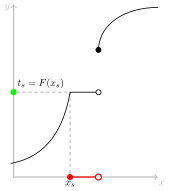
\includegraphics{distributionFunction}
        \caption{Ejemplo de funci\'on de distribuci\'on de probabilidad. En rojo se muestra la inversa $F^{-1}(t_s)$.}
	\label{f:cdf1D}
\end{figure}

Sea $S:= \{x_1, \ldots, x_n\}$ el conjunto formado por observaciones (valores medidos o muestreados) de la variable aleatoria $X$. Entonces se pueden estimar los valores de la funci\'on de distribuci\'on $F$ a partir de su funci\'on de distribuci\'on emp\'irica.

\begin{equation}
\label{e:empF} % "e"quation of the "Emp"irical Distribution function Fn.
\hat{F_n} (x) = \frac{1}{n}\sum_{k=1}^{n} \mathbbm{1} (x_k \le x)
\end{equation}

\noindent
donde $\mathbbm{1}$ es la funci\'on indicador (\autoref{e:indicatorFunc}) y $n$ es la cantidad de datos.

Esta funci\'on emp\'irica es la funci\'on no param\'etrica aproximante m\'as conocida de una funci\'on de distribuci\'on, pero tambi\'en existen otras como la de Weibull plotting position \'o est\'andar \citep[p. 10]{salvadori_extremes_2007}.
No se debe confundir con la unci\'on de densidad de Weibull, la cual es continua. En este trabajo utilizaremos la \autoref{e:empF} debido a su simplicidad y a su similitud con la c\'opula emp\'irica que se ver\'a m\'as adelante.

A partir de ahora, en lo que resta de esta subsecci\'on, supondremos que los datos observados $x_i$ est\'an ordenados en orden creciente ($x_i < x_{i+1}$) y no hay datos duplicados, es decir, que los datos son iguales a sus estad\'isticos de orden $x_{(i)}$.

El gr\'afico de la funci\'on de distribuci\'on emp\'irica (\autoref{f:empCDF}) es constante a tramos con saltos de magnitud $1/n$ cada $x_i$.
%En cada salto, los puntos rellenos representan un punto en la curva $\hat{F_n}$ mientras que los puntos vac\'ios representan un punto que \textit{no} pertenece a la funci\'on de distribuci\'on emp\'irica.
Si definimos las \textbf{pseudo-observaciones} como $u_i := \hat{F_n}(x_i)$,
%entonces los puntos rellenos tienen coordenadas $(x_i, u_i)$.
interpretada como una probabilidad en el intervalo $[0,1]$, $u_i$ es una cantidad adimensional.

\begin{figure}[H]
	\centering
	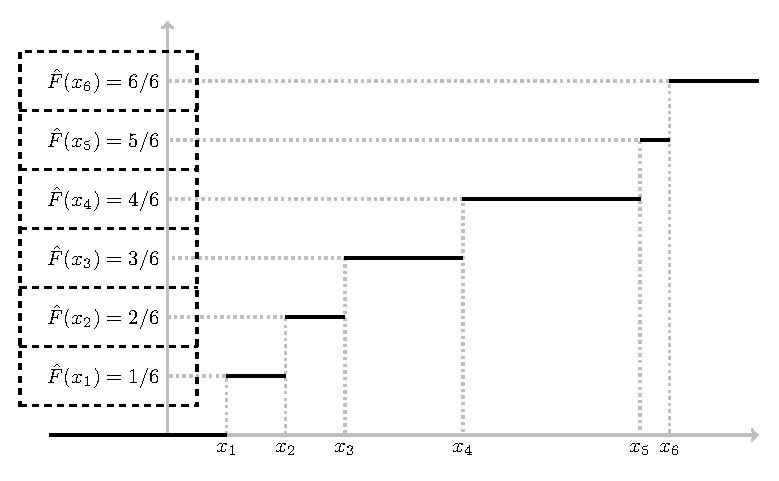
\includegraphics{empCDF}
	\caption{Funci\'on de distribuci\'on emp\'irica. Los rect\'angulos en negro con l\'ineas de guiones se muestra el correspondiente arreglo computacional para almacenar los valores de $\hat{F}_n$.}
	\label{f:empCDF}
\end{figure}

Desde el punto de vista computacional, para obtener valores de esta funci\'on emp\'irica solamente basta con almacenar los valores de $\hat{F}_n(x_i)$, para toda $i=1,\ldots, n$.

$$
\begin{array}{| c | c | c | c | c | c |}
	\hline
	\hat{F}_n(x_1) & \hat{F}_n(x_2) & \hat{F}_n(x_3) & \cdots & \hat{F}_n(x_{n-1}) & \hat{F}_n(x_n) \\ \hline
\end{array}
$$

De esta manera para saber el valor de $\hat{F}_n$ en cualquier otro valor $x$, solamente hay que compararlo contra todas las observaciones y saber cu\'al $x_i$ es el inmediato inferior.
Esto es lo que significa la \autoref{e:empF}: para obtener un valor $\hat{F}(x)$, $x$ se compara con cada observaci\'on $x_i$.
N\'otese que ya no se requieren los valores $x_i$ ya que est\'an impl\'icitos en vector de valores de $\hat{F}_n$, solamente es necesario saber cu\'al es el \'indice $i$ para poder acceder al arreglo.
Para lenguajes de programaci\'on de bajo nivel como C/C++ o Fortran, esto se pudiera implementar en un arreglo de enteros sin signo, lo que reduce el uso de memoria comparado con un arreglo de n\'umeros reales (valores flotantes).
Los \'indices de la \autoref{f:empCDF} corresponden uno-a-uno con arreglos de lenguajes de programaci\'on con offset $1$ como R o Matlab, pero no para arreglos de lenguajes programaci\'on de offset $0$ como Python o C++.
A\'un m\'as, pudiera ahorrarse guardar tal arreglo ya que el c\'alculo de $1/i$ es computacionalmente muy r\'apido.

La implementaci\'on computacional de la funci\'on de distribuci\'on emp\'irica est\'a en la funci\'on \verb|stats::ecdf| del software \verb|R|.

Como puede verse en la \autoref{f:empCDF}, la funci\'on de distribuci\'on emp\'irica no es continua, pero existen muchos modelos que s\'i lo son. Por ejemplo, se encuentran la funci\'on normal, la lognormal, ley de potencias, Weibull, exponencial, entre otras. Estos ejemplos, salvo la distribuci\'on normal, tienen asimetr\'ia positiva, y son com\'unmente utilizadas en el modelado de las longitudes de fracturas \citep{bonnet_scaling_2001,bour_connectivity_1997,gudmundsson_power-law_2011}. Aunque estas distribuciones dependen de ciertos par\'ametros (la media y la varianza en el caso de la distribuci\'on normal), tambi\'en existen funciones de distribuci\'on no param\'etricas. Otras variables que pueden ser modeladas con dichas funciones son la apertura, la porosidad y la permeabilidad.

En muchas ocasiones unos de los objetivos buscados mediante el an\'alisis y modelado de los datos es la simulaci\'on, ya que permite cuantificar la incertidumbre del fen\'omeno. Un algoritmo de simulaci\'on denominado de la transformada inversa requiere la funci\'on cuantil. \'Esta es una funci\'on asociada con una variable aleatoria $X$, la cual se define como la inversa generalizada $F^-:[0,1] \to \overline{\mathbb{R}}= [-\infty, \infty]$ de la funci\'on de distribuci\'on $F$ \citep{embrechts_note_2013}:

\begin{equation}
	F^-(y)= \inf \{x \in \mathbb{R}:F(x) \ge y\}
	\label{e:generalizedInv}
\end{equation}

\noindent
con la convenci\'on que $\inf \emptyset = \infty$. Esta inversa puede visualizarse en la \autoref{f:cdf1D}. Si $F$ es estrictamente creciente, entonces $F^- = F^{-1}$, la inversa generalizada es igual a la inversa usual.

Dicha funci\'on cuantil, puede o no existir en forma expl\'icita independientemente si la funci\'on $F$ existe en forma expl\'icita. Por ejemplo, se tiene una f\'ormula algebraica para la funci\'on de densidad de la distribuci\'on normal pero no se tiene una para calcular la funci\'on de distribuci\'on o la funci\'on cuantil, para estos casos se tiene que recurrir a m\'etodos num\'ericos. Un ejemplo parecido es el encontrado con la funci\'on de densidad de von Mises (V\'ease \autoref{ss:circularStats}).

Un ejemplo opuesto se tiene con los polinomios de Bernstein-Kantorovich \citep{munoz-perez_estimating_1987}, que representan de forma semi-expl\'icita la funci\'on cuantil, pero para obtener su correspondiente funci\'on de distribuci\'on se tiene que recurrir a m\'etodos num\'ericos \citep{quarteroni_numerical_2006,dahlquist_numerical_2008}. Esta funci\'on no param\'etrica y continua es un caso particular de una curva de B\'ezier (ver \autoref{ch:approxTheory}). La implementaci\'on computacional de esta funci\'on puede ser utilizada mediante la funci\'on \verb|lmomco::dat2bernqua| \citep{asquith_lmomco:_2017}.

Encontrar num\'ericamente la inversa de una funci\'on $F$ para un valor $y$ en su imagen, es equivalente a encontrar la ra\'iz $x$ de la funci\'on $G(x,y)= F(x) - y = 0$. Una implementaci\'on computacional para encontrar dicha ra\'iz se puede encontrar en el software R con la funci\'on \verb|stats::uniroot|. Otra funci\'on que podr\'ia ser m\'as r\'apida es utilizando una versi\'on paralelizada del m\'etodo de bisecci\'on para encontrar dicha ra\'iz \citep{miranker_survey_1971,nijmeijer_parallel_2015,stack_overflow_algorithm_2017,karniadakis_parallel_2003}. Tambi\'en se puede aprovechar el hecho de que la funci\'on $G$, debido a que es una traslaci\'on de $F$, es mon\'otona.


% \chapter{Estad\'istica de datos orientados}
\label{ch:prob}

Antes de revisar el tema principal de este cap\'itulo es conveniente revisar algunos temas de probabilidad que son comunes o equivalentes.

\section{Variables aleatorias}
\label{s:randomVar}

Una variable aleatoria es una funci\'on en donde el dominio es un espacio de posibles opciones $S$ y la imagen son los n\'umeros reales $\mathbb{R}$ \citep{casella_statistical_2002}.
El t\'ermino \textit{aleatorio} en la definici\'on hace referencia a la ley probabilidad y no significa que tenga la misma probabilidad en cualquier intervalo de su imagen. A largo de este escrito se entender\'a de esta manera.

\textit{Notaci\'on}: Las variables aleatorias se denotar\'an con letras may\'usculas, $X$ por ejemplo. Por otro lado, las realizaciones/observaciones de esta variable aleatoria (o su imagen) ser\'an denotadas con las correspondientes letras min\'usculas, $x$ para el ejemplo anterior. A diferencia del cap\'itulo anterior en que $x$ y $X$ indicaban ubicaci\'on espacial, en este cap\'itulo y el que sigue se utilizar\'a para referirnos a una variable aleatoria.
%Como ejemplo m\'as espec\'ifico tenemos el siguiente: $X$, la estatura de los mexicanos, puede tomar el valor $x=1.7$ m.

El objeto de estudio de este proyecto doctoral fueron fen\'omenos que se modelaron con variables aleatorias continuas, es decir, variables aleatorias cuya imagen pod\'ia tomar cualquier valor dentro de cierto intervalo no nulo de los reales.

Las funciones aleatorias son completamente caracterizadas por su funci\'on de distribuci\'on de probabilidad $F$, tambi\'en conocidas como funci\'on de distribuci\'on acumulativa (CDF, por sus siglas en ingl\'es):

\begin{equation}
	F_X(x) = P_X(X \le x), \qquad \forall x. 
	\label{e:cdf1D}
\end{equation}

\noindent
donde $P$ denota la probabilidad de que la variable aleatoria $X$ sea menor o igual que el valor $x$.
%Por ejemplo, la probabilidad de que la estatura, $X$, sea menor que $x = 1.5$ m.

Para caracterizar completamente una variable aleatoria continua $X$, alternativamente a la funci\'on de distribuci\'on $F$, se tiene la funci\'on de densidad de probabilidad $f$:

\begin{equation}
	F_X(x) = \int_{-\infty}^x f_X(t)dt \qquad \forall x.
\end{equation}

Si $f_X(x)$ es continua, entonces, por el teorema fundamental del c\'alculo:

\begin{equation}
	\frac{d}{dx}F_X(x) = f_X(x)
\end{equation}

El histograma es un estimador de la funci\'on de densidad $f_X$.

Para mostrar las caracter\'isticas de una CDF usemos la diferencia hacia adelante de primer orden:

\begin{equation}
\label{e:ForwDiff} % "Forw"ard "Diff"erence
\Delta F :=F(x+d)-F(x)
\end{equation}

Una funci\'on de distribuci\'on $F$ satisface las siguientes condiciones:

\begin{itemize}
	\item $F(x)$ es una funci\'on no-decreciente de $x$. Es decir, $\Delta F \ge 0$.
	\item $F(x)$ continua por la derecha. Es decir, para cada n\'umero $x_0$, $\lim_{x \to x_0^+}F(x) = F(x_0)$.
	\item $\lim_{x \to -\infty}F(x) = 0$, y  $\lim_{x \to +\infty}F(x) = 1$.
\end{itemize}

N\'otese que no hay significado probabil\'istico en estas definiciones, dicha interpretaci\'on se obtiene a partir de la definici\'on en la \autoref{e:cdf1D}. Gr\'aficamente, todas estas caracter\'isticas se pueden observar en la \autoref{f:cdf1D}.

\begin{figure}
	\centering
	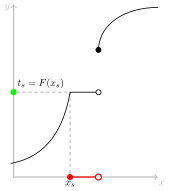
\includegraphics{distributionFunction}
        \caption{Ejemplo de funci\'on de distribuci\'on de probabilidad. En rojo se muestra la inversa $F^{-1}(t_s)$.}
	\label{f:cdf1D}
\end{figure}

Sea $S:= \{x_1, \ldots, x_n\}$ el conjunto formado por observaciones (valores medidos o muestreados) de la variable aleatoria $X$. Entonces se pueden estimar los valores de la funci\'on de distribuci\'on $F$ a partir de su funci\'on de distribuci\'on emp\'irica.

\begin{equation}
\label{e:empF} % "e"quation of the "Emp"irical Distribution function Fn.
\hat{F_n} (x) = \frac{1}{n}\sum_{k=1}^{n} \mathbbm{1} (x_k \le x)
\end{equation}

\noindent
donde $\mathbbm{1}$ es la funci\'on indicador (\autoref{e:indicatorFunc}) y $n$ es la cantidad de datos.

Esta funci\'on emp\'irica es la funci\'on no param\'etrica aproximante m\'as conocida de una funci\'on de distribuci\'on, pero tambi\'en existen otras como la de Weibull plotting position \'o est\'andar \citep[p. 10]{salvadori_extremes_2007}.
No se debe confundir con la unci\'on de densidad de Weibull, la cual es continua. En este trabajo utilizaremos la \autoref{e:empF} debido a su simplicidad y a su similitud con la c\'opula emp\'irica que se ver\'a m\'as adelante.

A partir de ahora, en lo que resta de esta subsecci\'on, supondremos que los datos observados $x_i$ est\'an ordenados en orden creciente ($x_i < x_{i+1}$) y no hay datos duplicados, es decir, que los datos son iguales a sus estad\'isticos de orden $x_{(i)}$.

El gr\'afico de la funci\'on de distribuci\'on emp\'irica (\autoref{f:empCDF}) es constante a tramos con saltos de magnitud $1/n$ cada $x_i$.
%En cada salto, los puntos rellenos representan un punto en la curva $\hat{F_n}$ mientras que los puntos vac\'ios representan un punto que \textit{no} pertenece a la funci\'on de distribuci\'on emp\'irica.
Si definimos las \textbf{pseudo-observaciones} como $u_i := \hat{F_n}(x_i)$,
%entonces los puntos rellenos tienen coordenadas $(x_i, u_i)$.
interpretada como una probabilidad en el intervalo $[0,1]$, $u_i$ es una cantidad adimensional.

\begin{figure}[H]
	\centering
	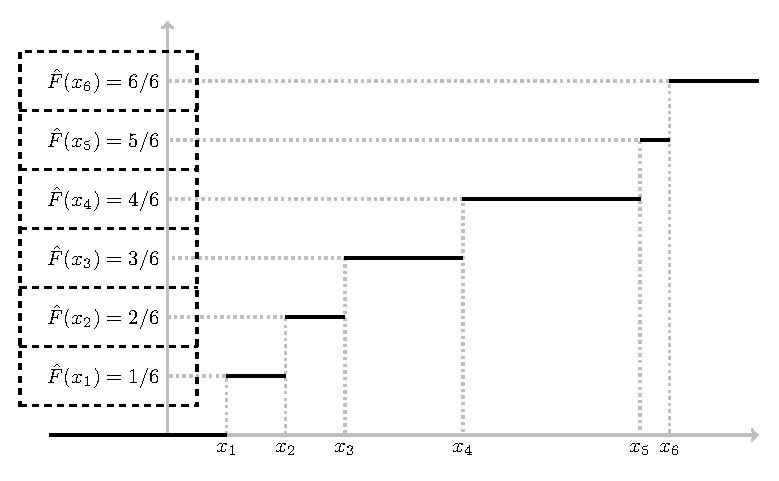
\includegraphics{empCDF}
	\caption{Funci\'on de distribuci\'on emp\'irica. Los rect\'angulos en negro con l\'ineas de guiones se muestra el correspondiente arreglo computacional para almacenar los valores de $\hat{F}_n$.}
	\label{f:empCDF}
\end{figure}

Desde el punto de vista computacional, para obtener valores de esta funci\'on emp\'irica solamente basta con almacenar los valores de $\hat{F}_n(x_i)$, para toda $i=1,\ldots, n$.

$$
\begin{array}{| c | c | c | c | c | c |}
	\hline
	\hat{F}_n(x_1) & \hat{F}_n(x_2) & \hat{F}_n(x_3) & \cdots & \hat{F}_n(x_{n-1}) & \hat{F}_n(x_n) \\ \hline
\end{array}
$$

De esta manera para saber el valor de $\hat{F}_n$ en cualquier otro valor $x$, solamente hay que compararlo contra todas las observaciones y saber cu\'al $x_i$ es el inmediato inferior.
Esto es lo que significa la \autoref{e:empF}: para obtener un valor $\hat{F}(x)$, $x$ se compara con cada observaci\'on $x_i$.
N\'otese que ya no se requieren los valores $x_i$ ya que est\'an impl\'icitos en vector de valores de $\hat{F}_n$, solamente es necesario saber cu\'al es el \'indice $i$ para poder acceder al arreglo.
Para lenguajes de programaci\'on de bajo nivel como C/C++ o Fortran, esto se pudiera implementar en un arreglo de enteros sin signo, lo que reduce el uso de memoria comparado con un arreglo de n\'umeros reales (valores flotantes).
Los \'indices de la \autoref{f:empCDF} corresponden uno-a-uno con arreglos de lenguajes de programaci\'on con offset $1$ como R o Matlab, pero no para arreglos de lenguajes programaci\'on de offset $0$ como Python o C++.
A\'un m\'as, pudiera ahorrarse guardar tal arreglo ya que el c\'alculo de $1/i$ es computacionalmente muy r\'apido.

La implementaci\'on computacional de la funci\'on de distribuci\'on emp\'irica est\'a en la funci\'on \verb|stats::ecdf| del software \verb|R|.

Como puede verse en la \autoref{f:empCDF}, la funci\'on de distribuci\'on emp\'irica no es continua, pero existen muchos modelos que s\'i lo son. Por ejemplo, se encuentran la funci\'on normal, la lognormal, ley de potencias, Weibull, exponencial, entre otras. Estos ejemplos, salvo la distribuci\'on normal, tienen asimetr\'ia positiva, y son com\'unmente utilizadas en el modelado de las longitudes de fracturas \citep{bonnet_scaling_2001,bour_connectivity_1997,gudmundsson_power-law_2011}. Aunque estas distribuciones dependen de ciertos par\'ametros (la media y la varianza en el caso de la distribuci\'on normal), tambi\'en existen funciones de distribuci\'on no param\'etricas. Otras variables que pueden ser modeladas con dichas funciones son la apertura, la porosidad y la permeabilidad.

En muchas ocasiones unos de los objetivos buscados mediante el an\'alisis y modelado de los datos es la simulaci\'on, ya que permite cuantificar la incertidumbre del fen\'omeno. Un algoritmo de simulaci\'on denominado de la transformada inversa requiere la funci\'on cuantil. \'Esta es una funci\'on asociada con una variable aleatoria $X$, la cual se define como la inversa generalizada $F^-:[0,1] \to \overline{\mathbb{R}}= [-\infty, \infty]$ de la funci\'on de distribuci\'on $F$ \citep{embrechts_note_2013}:

\begin{equation}
	F^-(y)= \inf \{x \in \mathbb{R}:F(x) \ge y\}
	\label{e:generalizedInv}
\end{equation}

\noindent
con la convenci\'on que $\inf \emptyset = \infty$. Esta inversa puede visualizarse en la \autoref{f:cdf1D}. Si $F$ es estrictamente creciente, entonces $F^- = F^{-1}$, la inversa generalizada es igual a la inversa usual.

Dicha funci\'on cuantil, puede o no existir en forma expl\'icita independientemente si la funci\'on $F$ existe en forma expl\'icita. Por ejemplo, se tiene una f\'ormula algebraica para la funci\'on de densidad de la distribuci\'on normal pero no se tiene una para calcular la funci\'on de distribuci\'on o la funci\'on cuantil, para estos casos se tiene que recurrir a m\'etodos num\'ericos. Un ejemplo parecido es el encontrado con la funci\'on de densidad de von Mises (V\'ease \autoref{ss:circularStats}).

Un ejemplo opuesto se tiene con los polinomios de Bernstein-Kantorovich \citep{munoz-perez_estimating_1987}, que representan de forma semi-expl\'icita la funci\'on cuantil, pero para obtener su correspondiente funci\'on de distribuci\'on se tiene que recurrir a m\'etodos num\'ericos \citep{quarteroni_numerical_2006,dahlquist_numerical_2008}. Esta funci\'on no param\'etrica y continua es un caso particular de una curva de B\'ezier (ver \autoref{ch:approxTheory}). La implementaci\'on computacional de esta funci\'on puede ser utilizada mediante la funci\'on \verb|lmomco::dat2bernqua| \citep{asquith_lmomco:_2017}.

Encontrar num\'ericamente la inversa de una funci\'on $F$ para un valor $y$ en su imagen, es equivalente a encontrar la ra\'iz $x$ de la funci\'on $G(x,y)= F(x) - y = 0$. Una implementaci\'on computacional para encontrar dicha ra\'iz se puede encontrar en el software R con la funci\'on \verb|stats::uniroot|. Otra funci\'on que podr\'ia ser m\'as r\'apida es utilizando una versi\'on paralelizada del m\'etodo de bisecci\'on para encontrar dicha ra\'iz \citep{miranker_survey_1971,nijmeijer_parallel_2015,stack_overflow_algorithm_2017,karniadakis_parallel_2003}. Tambi\'en se puede aprovechar el hecho de que la funci\'on $G$, debido a que es una traslaci\'on de $F$, es mon\'otona.


% \chapter{Estad\'istica de datos orientados}
\label{ch:prob}

Antes de revisar el tema principal de este cap\'itulo es conveniente revisar algunos temas de probabilidad que son comunes o equivalentes.

\section{Variables aleatorias}
\label{s:randomVar}

Una variable aleatoria es una funci\'on en donde el dominio es un espacio de posibles opciones $S$ y la imagen son los n\'umeros reales $\mathbb{R}$ \citep{casella_statistical_2002}.
El t\'ermino \textit{aleatorio} en la definici\'on hace referencia a la ley probabilidad y no significa que tenga la misma probabilidad en cualquier intervalo de su imagen. A largo de este escrito se entender\'a de esta manera.

\textit{Notaci\'on}: Las variables aleatorias se denotar\'an con letras may\'usculas, $X$ por ejemplo. Por otro lado, las realizaciones/observaciones de esta variable aleatoria (o su imagen) ser\'an denotadas con las correspondientes letras min\'usculas, $x$ para el ejemplo anterior. A diferencia del cap\'itulo anterior en que $x$ y $X$ indicaban ubicaci\'on espacial, en este cap\'itulo y el que sigue se utilizar\'a para referirnos a una variable aleatoria.
%Como ejemplo m\'as espec\'ifico tenemos el siguiente: $X$, la estatura de los mexicanos, puede tomar el valor $x=1.7$ m.

El objeto de estudio de este proyecto doctoral fueron fen\'omenos que se modelaron con variables aleatorias continuas, es decir, variables aleatorias cuya imagen pod\'ia tomar cualquier valor dentro de cierto intervalo no nulo de los reales.

Las funciones aleatorias son completamente caracterizadas por su funci\'on de distribuci\'on de probabilidad $F$, tambi\'en conocidas como funci\'on de distribuci\'on acumulativa (CDF, por sus siglas en ingl\'es):

\begin{equation}
	F_X(x) = P_X(X \le x), \qquad \forall x. 
	\label{e:cdf1D}
\end{equation}

\noindent
donde $P$ denota la probabilidad de que la variable aleatoria $X$ sea menor o igual que el valor $x$.
%Por ejemplo, la probabilidad de que la estatura, $X$, sea menor que $x = 1.5$ m.

Para caracterizar completamente una variable aleatoria continua $X$, alternativamente a la funci\'on de distribuci\'on $F$, se tiene la funci\'on de densidad de probabilidad $f$:

\begin{equation}
	F_X(x) = \int_{-\infty}^x f_X(t)dt \qquad \forall x.
\end{equation}

Si $f_X(x)$ es continua, entonces, por el teorema fundamental del c\'alculo:

\begin{equation}
	\frac{d}{dx}F_X(x) = f_X(x)
\end{equation}

El histograma es un estimador de la funci\'on de densidad $f_X$.

Para mostrar las caracter\'isticas de una CDF usemos la diferencia hacia adelante de primer orden:

\begin{equation}
\label{e:ForwDiff} % "Forw"ard "Diff"erence
\Delta F :=F(x+d)-F(x)
\end{equation}

Una funci\'on de distribuci\'on $F$ satisface las siguientes condiciones:

\begin{itemize}
	\item $F(x)$ es una funci\'on no-decreciente de $x$. Es decir, $\Delta F \ge 0$.
	\item $F(x)$ continua por la derecha. Es decir, para cada n\'umero $x_0$, $\lim_{x \to x_0^+}F(x) = F(x_0)$.
	\item $\lim_{x \to -\infty}F(x) = 0$, y  $\lim_{x \to +\infty}F(x) = 1$.
\end{itemize}

N\'otese que no hay significado probabil\'istico en estas definiciones, dicha interpretaci\'on se obtiene a partir de la definici\'on en la \autoref{e:cdf1D}. Gr\'aficamente, todas estas caracter\'isticas se pueden observar en la \autoref{f:cdf1D}.

\begin{figure}
	\centering
	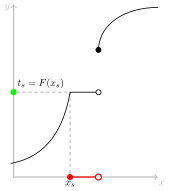
\includegraphics{distributionFunction}
        \caption{Ejemplo de funci\'on de distribuci\'on de probabilidad. En rojo se muestra la inversa $F^{-1}(t_s)$.}
	\label{f:cdf1D}
\end{figure}

Sea $S:= \{x_1, \ldots, x_n\}$ el conjunto formado por observaciones (valores medidos o muestreados) de la variable aleatoria $X$. Entonces se pueden estimar los valores de la funci\'on de distribuci\'on $F$ a partir de su funci\'on de distribuci\'on emp\'irica.

\begin{equation}
\label{e:empF} % "e"quation of the "Emp"irical Distribution function Fn.
\hat{F_n} (x) = \frac{1}{n}\sum_{k=1}^{n} \mathbbm{1} (x_k \le x)
\end{equation}

\noindent
donde $\mathbbm{1}$ es la funci\'on indicador (\autoref{e:indicatorFunc}) y $n$ es la cantidad de datos.

Esta funci\'on emp\'irica es la funci\'on no param\'etrica aproximante m\'as conocida de una funci\'on de distribuci\'on, pero tambi\'en existen otras como la de Weibull plotting position \'o est\'andar \citep[p. 10]{salvadori_extremes_2007}.
No se debe confundir con la unci\'on de densidad de Weibull, la cual es continua. En este trabajo utilizaremos la \autoref{e:empF} debido a su simplicidad y a su similitud con la c\'opula emp\'irica que se ver\'a m\'as adelante.

A partir de ahora, en lo que resta de esta subsecci\'on, supondremos que los datos observados $x_i$ est\'an ordenados en orden creciente ($x_i < x_{i+1}$) y no hay datos duplicados, es decir, que los datos son iguales a sus estad\'isticos de orden $x_{(i)}$.

El gr\'afico de la funci\'on de distribuci\'on emp\'irica (\autoref{f:empCDF}) es constante a tramos con saltos de magnitud $1/n$ cada $x_i$.
%En cada salto, los puntos rellenos representan un punto en la curva $\hat{F_n}$ mientras que los puntos vac\'ios representan un punto que \textit{no} pertenece a la funci\'on de distribuci\'on emp\'irica.
Si definimos las \textbf{pseudo-observaciones} como $u_i := \hat{F_n}(x_i)$,
%entonces los puntos rellenos tienen coordenadas $(x_i, u_i)$.
interpretada como una probabilidad en el intervalo $[0,1]$, $u_i$ es una cantidad adimensional.

\begin{figure}[H]
	\centering
	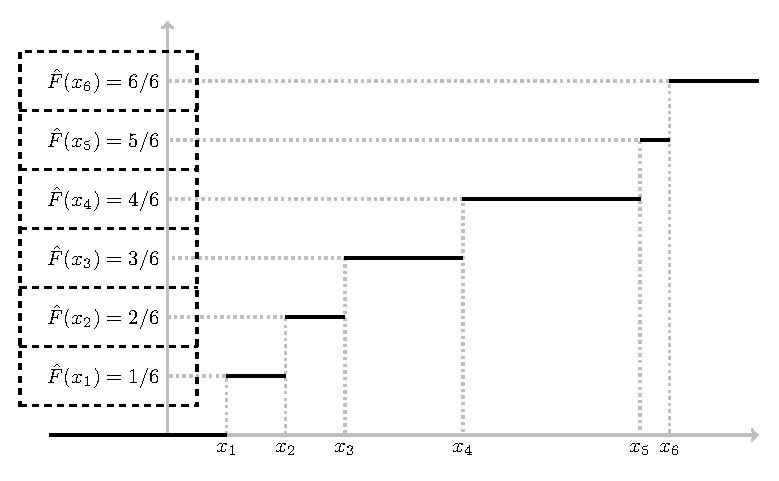
\includegraphics{empCDF}
	\caption{Funci\'on de distribuci\'on emp\'irica. Los rect\'angulos en negro con l\'ineas de guiones se muestra el correspondiente arreglo computacional para almacenar los valores de $\hat{F}_n$.}
	\label{f:empCDF}
\end{figure}

Desde el punto de vista computacional, para obtener valores de esta funci\'on emp\'irica solamente basta con almacenar los valores de $\hat{F}_n(x_i)$, para toda $i=1,\ldots, n$.

$$
\begin{array}{| c | c | c | c | c | c |}
	\hline
	\hat{F}_n(x_1) & \hat{F}_n(x_2) & \hat{F}_n(x_3) & \cdots & \hat{F}_n(x_{n-1}) & \hat{F}_n(x_n) \\ \hline
\end{array}
$$

De esta manera para saber el valor de $\hat{F}_n$ en cualquier otro valor $x$, solamente hay que compararlo contra todas las observaciones y saber cu\'al $x_i$ es el inmediato inferior.
Esto es lo que significa la \autoref{e:empF}: para obtener un valor $\hat{F}(x)$, $x$ se compara con cada observaci\'on $x_i$.
N\'otese que ya no se requieren los valores $x_i$ ya que est\'an impl\'icitos en vector de valores de $\hat{F}_n$, solamente es necesario saber cu\'al es el \'indice $i$ para poder acceder al arreglo.
Para lenguajes de programaci\'on de bajo nivel como C/C++ o Fortran, esto se pudiera implementar en un arreglo de enteros sin signo, lo que reduce el uso de memoria comparado con un arreglo de n\'umeros reales (valores flotantes).
Los \'indices de la \autoref{f:empCDF} corresponden uno-a-uno con arreglos de lenguajes de programaci\'on con offset $1$ como R o Matlab, pero no para arreglos de lenguajes programaci\'on de offset $0$ como Python o C++.
A\'un m\'as, pudiera ahorrarse guardar tal arreglo ya que el c\'alculo de $1/i$ es computacionalmente muy r\'apido.

La implementaci\'on computacional de la funci\'on de distribuci\'on emp\'irica est\'a en la funci\'on \verb|stats::ecdf| del software \verb|R|.

Como puede verse en la \autoref{f:empCDF}, la funci\'on de distribuci\'on emp\'irica no es continua, pero existen muchos modelos que s\'i lo son. Por ejemplo, se encuentran la funci\'on normal, la lognormal, ley de potencias, Weibull, exponencial, entre otras. Estos ejemplos, salvo la distribuci\'on normal, tienen asimetr\'ia positiva, y son com\'unmente utilizadas en el modelado de las longitudes de fracturas \citep{bonnet_scaling_2001,bour_connectivity_1997,gudmundsson_power-law_2011}. Aunque estas distribuciones dependen de ciertos par\'ametros (la media y la varianza en el caso de la distribuci\'on normal), tambi\'en existen funciones de distribuci\'on no param\'etricas. Otras variables que pueden ser modeladas con dichas funciones son la apertura, la porosidad y la permeabilidad.

En muchas ocasiones unos de los objetivos buscados mediante el an\'alisis y modelado de los datos es la simulaci\'on, ya que permite cuantificar la incertidumbre del fen\'omeno. Un algoritmo de simulaci\'on denominado de la transformada inversa requiere la funci\'on cuantil. \'Esta es una funci\'on asociada con una variable aleatoria $X$, la cual se define como la inversa generalizada $F^-:[0,1] \to \overline{\mathbb{R}}= [-\infty, \infty]$ de la funci\'on de distribuci\'on $F$ \citep{embrechts_note_2013}:

\begin{equation}
	F^-(y)= \inf \{x \in \mathbb{R}:F(x) \ge y\}
	\label{e:generalizedInv}
\end{equation}

\noindent
con la convenci\'on que $\inf \emptyset = \infty$. Esta inversa puede visualizarse en la \autoref{f:cdf1D}. Si $F$ es estrictamente creciente, entonces $F^- = F^{-1}$, la inversa generalizada es igual a la inversa usual.

Dicha funci\'on cuantil, puede o no existir en forma expl\'icita independientemente si la funci\'on $F$ existe en forma expl\'icita. Por ejemplo, se tiene una f\'ormula algebraica para la funci\'on de densidad de la distribuci\'on normal pero no se tiene una para calcular la funci\'on de distribuci\'on o la funci\'on cuantil, para estos casos se tiene que recurrir a m\'etodos num\'ericos. Un ejemplo parecido es el encontrado con la funci\'on de densidad de von Mises (V\'ease \autoref{ss:circularStats}).

Un ejemplo opuesto se tiene con los polinomios de Bernstein-Kantorovich \citep{munoz-perez_estimating_1987}, que representan de forma semi-expl\'icita la funci\'on cuantil, pero para obtener su correspondiente funci\'on de distribuci\'on se tiene que recurrir a m\'etodos num\'ericos \citep{quarteroni_numerical_2006,dahlquist_numerical_2008}. Esta funci\'on no param\'etrica y continua es un caso particular de una curva de B\'ezier (ver \autoref{ch:approxTheory}). La implementaci\'on computacional de esta funci\'on puede ser utilizada mediante la funci\'on \verb|lmomco::dat2bernqua| \citep{asquith_lmomco:_2017}.

Encontrar num\'ericamente la inversa de una funci\'on $F$ para un valor $y$ en su imagen, es equivalente a encontrar la ra\'iz $x$ de la funci\'on $G(x,y)= F(x) - y = 0$. Una implementaci\'on computacional para encontrar dicha ra\'iz se puede encontrar en el software R con la funci\'on \verb|stats::uniroot|. Otra funci\'on que podr\'ia ser m\'as r\'apida es utilizando una versi\'on paralelizada del m\'etodo de bisecci\'on para encontrar dicha ra\'iz \citep{miranker_survey_1971,nijmeijer_parallel_2015,stack_overflow_algorithm_2017,karniadakis_parallel_2003}. Tambi\'en se puede aprovechar el hecho de que la funci\'on $G$, debido a que es una traslaci\'on de $F$, es mon\'otona.


% \include{TeX/directionalStats}

\section{Variables orientadas}
\label{ss:circularStats}

Los \emph{datos direccionales} (tambi\'en conocidos como \emph{datos orientados}) surgen de varias maneras. En particular, cuando se trata de una dimensi\'on (una sola variable aleatoria) se les llama \emph{datos circulares} y esta variable se encuentra definida sobre el c\'irculo unitario, \(\mathbb{S}^{1} = [0, 2 \pi) \). N\'otese que \'esta es una variable aleatoria con periodo \(2\pi\). Algunos ejemplos de variables aleatorias peri\'odicas son la direcci\'on de una br\'ujula (como direcci\'on del viento, direcci\'on del vuelo, direcci\'on de rumbo, etc.), la posici\'on de las manecillas del reloj, la temperatura diurna, o la anual, etc.

En la caracterizaci\'on de fracturas o fallas geol\'ogicas, se cuenta con datos cuya caracter\'istica es tener dos componentes de este estilo. Estas componentes son el \emph{echado} y \emph{azimut}; ambas asociadas a un solo dato y ambas medidas en \'angulos. Estas dos componentes generan un vector (o dato) en 3D, por lo que la herramienta que se deber\'ia considerar para el an\'alisis estad\'istico son los \emph{datos esf\'ericos} \cite{fisher_statistical_1993,jammalamadaka_topics_2001}.

En el caso univariado, la estad\'istica de datos orientados surge de manera natural si se intenta calcular la media y la desviaci\'on est\'andar del conjunto de datos que se muestra en la Figura 1. N\'otese que, si se calcula el promedio usual, el valor estimado para la media ser\'ia de 180$^\circ$~=~(10+350)/2, la cual es una direcci\'on diametralmente opuesta a la sugerida por los datos (0$^\circ$~= Este geogr\'afico). Tambi\'en n\'otese que si se procede con este camino la varianza correspondiente tambi\'en discrepa mucho de lo que se observa en el \emph{histograma circular} de la izquierda de la figura.


\begin{figure}[H]
	\centering 
\includegraphics[width=4.30250in,height=1.46419in]{directional_histogram}
	\caption{Motivaci\'on de la estad\'istica de datos orientados. \textquestiondown Cu\'al es la media? \textquestiondown Y la desviaci\'on est\'andar?}
	\label{f:directionalHist}
\end{figure}

La soluci\'on a este problema lo proporciona la estad\'istica de datos orientados al hacer uso del c\'alculo vectorial. Con este enfoque los estad\'igrafos b\'asicos para datos circulares se definen de la siguiente manera \citep[ch. 2]{mardia_directional_2000} y est\'an implementados en el paquete \verb|circular| del software estad\'istico \verb|R|:

Supongamos que se tienen \(n\) datos, si cada orientaci\'on \(\theta_{i}\) se puede hacer corresponder con un vector unitario \(\mathbf{x}_{\mathbf{i}} = ( \cos\theta_{i},\sin\theta_{i} )\); entonces la direcci\'on media \(\overline{\theta}\) es la direcci\'on del vector resultante \(\mathbf{x}_{\mathbf{1}} + \ldots + \mathbf{x}_{\mathbf{n}}\). Las coordenadas cartesianas del centro de masa son \(( \overline{C},\ \overline{S} )\), donde

\begin{equation}
\overline{C} = \frac{1}{n}\sum_{j = 1}^{n}{\cos\theta_{j}},
\quad
\overline{S} = \frac{1}{n}\sum_{j = 1}^{n}{\sin\theta_{j}}
\end{equation}

Por lo tanto \(\overline{\theta}\) es la soluci\'on a las ecuaciones

\begin{equation}
\overline{C} = \overline{R}\cos\overline{\theta},
\quad
\overline{S} = \overline{R}\operatorname{sen}\overline{\theta}\end{equation}

Donde la longitud resultante media \(\overline{R}\) est\'a dada por

\begin{equation}
\overline{R} = \sqrt{{\overline{C}}^{2} + {\overline{S}}^{2}} \end{equation}

Observe que \(0 \leq \overline{R} \leq 1\). Si las direcciones \(\theta_{1},\ldots,\theta_{n}\) son muy cercanas entre s\'i, entonces \(\overline{R}\) ser\'a cercano a 1, pero si est\'a muy dispersas entonces \(\overline{R}\) ser\'a cercano a 0. Por lo tanto \(\overline{R}\) es una medida de \emph{concentraci\'on} de los datos. N\'otese que en la \emph{estad\'istica convencional} (o de \emph{datos no orientados}), la varianza nos proporciona una medida de \emph{dispersi\'on}, opuesto a la interpretaci\'on de \(\overline{R}.\) An\'alogo a la varianza convencional y otros estad\'igrafos pueden encontrarse en el cap\'itulo 2 de \cite{mardia_directional_2000}. Para datos esf\'ericos o datos direccionales en \(\mathbb{R}^{p}\), consulte el cap\'itulo 9 del mismo libro o el libro de \cite{fisher_statistical_1993}.

Supongamos que se ha especificado una direcci\'on (origen) y orientaci\'on (sentido de giro) inicial. Dos ejemplos de tal especificaci\'on son: 1) un plano cartesiano matem\'atico (\(X^{+} = 0,\ Y^{+} = 90\)), y 2) uno geogr\'afico (N=0$^\circ$, E=90$^\circ$). Entonces la funci\'on de distribuci\'on \(F\) para un \'angulo aleatorio \(\theta\) se define como la funci\'on en
\(\mathbb{R}\) dada por

\[F( x ) = \mathrm{\Pr}( 0 < \theta \leq x )\]

\[0 \leq x \leq 2\pi\]

y

 \(F( x + 2\pi ) - F( x ) = 1\)
\(- \infty < x < \infty\) 

La ecuaci\'on significa que cualquier arco de longitud \(2\pi\) tiene probabilidad 1 (ya que tal arco es la totalidad de la circunferencia del c\'irculo).

A diferencia de distribuciones en los reales, \(\mathbb{R}\),

\[{F( x )} = \infty, \qquad
{F( x )} = - \infty\]

Por definici\'on,

\[F( 0 ) = 0, \qquad
F( 2\pi ) = 1\]

Para una variable circular, una funci\'on \(f\) es la densidad de probabilidad de una funci\'on de distribuci\'on totalmente (absolutely) continua si y s\'olo si

\begin{itemize}
\item
  \(f( \theta ) \geq 0\) casi por doquier en
  \(( - \infty,\infty )\),
\item
  \(f( \theta + 2k\pi ) = f( \theta )\) casi por
  doquier en \(( - \infty,\infty )\) con \(k\mathbb{\in Z}\)
  (i.e., \(f\) es peri\'odica),
\item
  \(\int_{0}^{2\pi}{f( \theta )\text{d}} = 1\).
\end{itemize}

Las funciones de densidad uni y bidimensional de probabilidad param\'etricas para datos orientados m\'as comunes son:

\begin{table}[H]
	\centering
	\label{tab:directionalModels}
	\begin{tabular}{|r|l|}
\hline
von Mises &
$f( \theta;\mu,\kappa ) = \frac{1}{2\pi I_{0}( \kappa )}e^{\kappa\cos( \theta - \mu )}$ \\
\hline
Fisher &
$f( \theta,\ \phi;\alpha,\beta,\ \kappa ) = \frac{1}{4\pi\sinh( \kappa )}\exp
[ \kappa\lbrack \operatorname{sen}\theta\operatorname{sen}\alpha\cos( \phi - \beta ) + \cos\theta\cos\alpha \rbrack ] \sin\theta$
\\ \hline
	\end{tabular}
	\caption{Funciones de densidad de probabilidad para datos orientados. $0 \le \theta < 2\pi, \quad 0 \le \phi < \pi/2,\quad 0 \le \kappa < \infty$. Ver ec. 3.5.17 de \cite{mardia_directional_2000}, ec. 2.2.6 en la secci\'on 2.2.4 de \cite{jammalamadaka_topics_2001} y ec. 4.22 de \cite{fisher_statistical_1993}.}
\end{table}

La funci\'on de densidad de von-Mises es el an\'alogo a la funci\'on de densidad de probabilidad normal ya que tambi\'en consta de dos par\'ametros, es unimodal y sim\'etrica.


\section{Variables orientadas}
\label{ss:circularStats}

Los \emph{datos direccionales} (tambi\'en conocidos como \emph{datos orientados}) surgen de varias maneras. En particular, cuando se trata de una dimensi\'on (una sola variable aleatoria) se les llama \emph{datos circulares} y esta variable se encuentra definida sobre el c\'irculo unitario, \(\mathbb{S}^{1} = [0, 2 \pi) \). N\'otese que \'esta es una variable aleatoria con periodo \(2\pi\). Algunos ejemplos de variables aleatorias peri\'odicas son la direcci\'on de una br\'ujula (como direcci\'on del viento, direcci\'on del vuelo, direcci\'on de rumbo, etc.), la posici\'on de las manecillas del reloj, la temperatura diurna, o la anual, etc.

En la caracterizaci\'on de fracturas o fallas geol\'ogicas, se cuenta con datos cuya caracter\'istica es tener dos componentes de este estilo. Estas componentes son el \emph{echado} y \emph{azimut}; ambas asociadas a un solo dato y ambas medidas en \'angulos. Estas dos componentes generan un vector (o dato) en 3D, por lo que la herramienta que se deber\'ia considerar para el an\'alisis estad\'istico son los \emph{datos esf\'ericos} \cite{fisher_statistical_1993,jammalamadaka_topics_2001}.

En el caso univariado, la estad\'istica de datos orientados surge de manera natural si se intenta calcular la media y la desviaci\'on est\'andar del conjunto de datos que se muestra en la Figura 1. N\'otese que, si se calcula el promedio usual, el valor estimado para la media ser\'ia de 180$^\circ$~=~(10+350)/2, la cual es una direcci\'on diametralmente opuesta a la sugerida por los datos (0$^\circ$~= Este geogr\'afico). Tambi\'en n\'otese que si se procede con este camino la varianza correspondiente tambi\'en discrepa mucho de lo que se observa en el \emph{histograma circular} de la izquierda de la figura.


\begin{figure}[H]
	\centering 
\includegraphics[width=4.30250in,height=1.46419in]{directional_histogram}
	\caption{Motivaci\'on de la estad\'istica de datos orientados. \textquestiondown Cu\'al es la media? \textquestiondown Y la desviaci\'on est\'andar?}
	\label{f:directionalHist}
\end{figure}

La soluci\'on a este problema lo proporciona la estad\'istica de datos orientados al hacer uso del c\'alculo vectorial. Con este enfoque los estad\'igrafos b\'asicos para datos circulares se definen de la siguiente manera \citep[ch. 2]{mardia_directional_2000} y est\'an implementados en el paquete \verb|circular| del software estad\'istico \verb|R|:

Supongamos que se tienen \(n\) datos, si cada orientaci\'on \(\theta_{i}\) se puede hacer corresponder con un vector unitario \(\mathbf{x}_{\mathbf{i}} = ( \cos\theta_{i},\sin\theta_{i} )\); entonces la direcci\'on media \(\overline{\theta}\) es la direcci\'on del vector resultante \(\mathbf{x}_{\mathbf{1}} + \ldots + \mathbf{x}_{\mathbf{n}}\). Las coordenadas cartesianas del centro de masa son \(( \overline{C},\ \overline{S} )\), donde

\begin{equation}
\overline{C} = \frac{1}{n}\sum_{j = 1}^{n}{\cos\theta_{j}},
\quad
\overline{S} = \frac{1}{n}\sum_{j = 1}^{n}{\sin\theta_{j}}
\end{equation}

Por lo tanto \(\overline{\theta}\) es la soluci\'on a las ecuaciones

\begin{equation}
\overline{C} = \overline{R}\cos\overline{\theta},
\quad
\overline{S} = \overline{R}\operatorname{sen}\overline{\theta}\end{equation}

Donde la longitud resultante media \(\overline{R}\) est\'a dada por

\begin{equation}
\overline{R} = \sqrt{{\overline{C}}^{2} + {\overline{S}}^{2}} \end{equation}

Observe que \(0 \leq \overline{R} \leq 1\). Si las direcciones \(\theta_{1},\ldots,\theta_{n}\) son muy cercanas entre s\'i, entonces \(\overline{R}\) ser\'a cercano a 1, pero si est\'a muy dispersas entonces \(\overline{R}\) ser\'a cercano a 0. Por lo tanto \(\overline{R}\) es una medida de \emph{concentraci\'on} de los datos. N\'otese que en la \emph{estad\'istica convencional} (o de \emph{datos no orientados}), la varianza nos proporciona una medida de \emph{dispersi\'on}, opuesto a la interpretaci\'on de \(\overline{R}.\) An\'alogo a la varianza convencional y otros estad\'igrafos pueden encontrarse en el cap\'itulo 2 de \cite{mardia_directional_2000}. Para datos esf\'ericos o datos direccionales en \(\mathbb{R}^{p}\), consulte el cap\'itulo 9 del mismo libro o el libro de \cite{fisher_statistical_1993}.

Supongamos que se ha especificado una direcci\'on (origen) y orientaci\'on (sentido de giro) inicial. Dos ejemplos de tal especificaci\'on son: 1) un plano cartesiano matem\'atico (\(X^{+} = 0,\ Y^{+} = 90\)), y 2) uno geogr\'afico (N=0$^\circ$, E=90$^\circ$). Entonces la funci\'on de distribuci\'on \(F\) para un \'angulo aleatorio \(\theta\) se define como la funci\'on en
\(\mathbb{R}\) dada por

\[F( x ) = \mathrm{\Pr}( 0 < \theta \leq x )\]

\[0 \leq x \leq 2\pi\]

y

 \(F( x + 2\pi ) - F( x ) = 1\)
\(- \infty < x < \infty\) 

La ecuaci\'on significa que cualquier arco de longitud \(2\pi\) tiene probabilidad 1 (ya que tal arco es la totalidad de la circunferencia del c\'irculo).

A diferencia de distribuciones en los reales, \(\mathbb{R}\),

\[{F( x )} = \infty, \qquad
{F( x )} = - \infty\]

Por definici\'on,

\[F( 0 ) = 0, \qquad
F( 2\pi ) = 1\]

Para una variable circular, una funci\'on \(f\) es la densidad de probabilidad de una funci\'on de distribuci\'on totalmente (absolutely) continua si y s\'olo si

\begin{itemize}
\item
  \(f( \theta ) \geq 0\) casi por doquier en
  \(( - \infty,\infty )\),
\item
  \(f( \theta + 2k\pi ) = f( \theta )\) casi por
  doquier en \(( - \infty,\infty )\) con \(k\mathbb{\in Z}\)
  (i.e., \(f\) es peri\'odica),
\item
  \(\int_{0}^{2\pi}{f( \theta )\text{d}} = 1\).
\end{itemize}

Las funciones de densidad uni y bidimensional de probabilidad param\'etricas para datos orientados m\'as comunes son:

\begin{table}[H]
	\centering
	\label{tab:directionalModels}
	\begin{tabular}{|r|l|}
\hline
von Mises &
$f( \theta;\mu,\kappa ) = \frac{1}{2\pi I_{0}( \kappa )}e^{\kappa\cos( \theta - \mu )}$ \\
\hline
Fisher &
$f( \theta,\ \phi;\alpha,\beta,\ \kappa ) = \frac{1}{4\pi\sinh( \kappa )}\exp
[ \kappa\lbrack \operatorname{sen}\theta\operatorname{sen}\alpha\cos( \phi - \beta ) + \cos\theta\cos\alpha \rbrack ] \sin\theta$
\\ \hline
	\end{tabular}
	\caption{Funciones de densidad de probabilidad para datos orientados. $0 \le \theta < 2\pi, \quad 0 \le \phi < \pi/2,\quad 0 \le \kappa < \infty$. Ver ec. 3.5.17 de \cite{mardia_directional_2000}, ec. 2.2.6 en la secci\'on 2.2.4 de \cite{jammalamadaka_topics_2001} y ec. 4.22 de \cite{fisher_statistical_1993}.}
\end{table}

La funci\'on de densidad de von-Mises es el an\'alogo a la funci\'on de densidad de probabilidad normal ya que tambi\'en consta de dos par\'ametros, es unimodal y sim\'etrica.


\section{Variables orientadas}
\label{ss:circularStats}

Los \emph{datos direccionales} (tambi\'en conocidos como \emph{datos orientados}) surgen de varias maneras. En particular, cuando se trata de una dimensi\'on (una sola variable aleatoria) se les llama \emph{datos circulares} y esta variable se encuentra definida sobre el c\'irculo unitario, \(\mathbb{S}^{1} = [0, 2 \pi) \). N\'otese que \'esta es una variable aleatoria con periodo \(2\pi\). Algunos ejemplos de variables aleatorias peri\'odicas son la direcci\'on de una br\'ujula (como direcci\'on del viento, direcci\'on del vuelo, direcci\'on de rumbo, etc.), la posici\'on de las manecillas del reloj, la temperatura diurna, o la anual, etc.

En la caracterizaci\'on de fracturas o fallas geol\'ogicas, se cuenta con datos cuya caracter\'istica es tener dos componentes de este estilo. Estas componentes son el \emph{echado} y \emph{azimut}; ambas asociadas a un solo dato y ambas medidas en \'angulos. Estas dos componentes generan un vector (o dato) en 3D, por lo que la herramienta que se deber\'ia considerar para el an\'alisis estad\'istico son los \emph{datos esf\'ericos} \cite{fisher_statistical_1993,jammalamadaka_topics_2001}.

En el caso univariado, la estad\'istica de datos orientados surge de manera natural si se intenta calcular la media y la desviaci\'on est\'andar del conjunto de datos que se muestra en la Figura 1. N\'otese que, si se calcula el promedio usual, el valor estimado para la media ser\'ia de 180$^\circ$~=~(10+350)/2, la cual es una direcci\'on diametralmente opuesta a la sugerida por los datos (0$^\circ$~= Este geogr\'afico). Tambi\'en n\'otese que si se procede con este camino la varianza correspondiente tambi\'en discrepa mucho de lo que se observa en el \emph{histograma circular} de la izquierda de la figura.


\begin{figure}[H]
	\centering 
\includegraphics[width=4.30250in,height=1.46419in]{directional_histogram}
	\caption{Motivaci\'on de la estad\'istica de datos orientados. \textquestiondown Cu\'al es la media? \textquestiondown Y la desviaci\'on est\'andar?}
	\label{f:directionalHist}
\end{figure}

La soluci\'on a este problema lo proporciona la estad\'istica de datos orientados al hacer uso del c\'alculo vectorial. Con este enfoque los estad\'igrafos b\'asicos para datos circulares se definen de la siguiente manera \citep[ch. 2]{mardia_directional_2000} y est\'an implementados en el paquete \verb|circular| del software estad\'istico \verb|R|:

Supongamos que se tienen \(n\) datos, si cada orientaci\'on \(\theta_{i}\) se puede hacer corresponder con un vector unitario \(\mathbf{x}_{\mathbf{i}} = ( \cos\theta_{i},\sin\theta_{i} )\); entonces la direcci\'on media \(\overline{\theta}\) es la direcci\'on del vector resultante \(\mathbf{x}_{\mathbf{1}} + \ldots + \mathbf{x}_{\mathbf{n}}\). Las coordenadas cartesianas del centro de masa son \(( \overline{C},\ \overline{S} )\), donde

\begin{equation}
\overline{C} = \frac{1}{n}\sum_{j = 1}^{n}{\cos\theta_{j}},
\quad
\overline{S} = \frac{1}{n}\sum_{j = 1}^{n}{\sin\theta_{j}}
\end{equation}

Por lo tanto \(\overline{\theta}\) es la soluci\'on a las ecuaciones

\begin{equation}
\overline{C} = \overline{R}\cos\overline{\theta},
\quad
\overline{S} = \overline{R}\operatorname{sen}\overline{\theta}\end{equation}

Donde la longitud resultante media \(\overline{R}\) est\'a dada por

\begin{equation}
\overline{R} = \sqrt{{\overline{C}}^{2} + {\overline{S}}^{2}} \end{equation}

Observe que \(0 \leq \overline{R} \leq 1\). Si las direcciones \(\theta_{1},\ldots,\theta_{n}\) son muy cercanas entre s\'i, entonces \(\overline{R}\) ser\'a cercano a 1, pero si est\'a muy dispersas entonces \(\overline{R}\) ser\'a cercano a 0. Por lo tanto \(\overline{R}\) es una medida de \emph{concentraci\'on} de los datos. N\'otese que en la \emph{estad\'istica convencional} (o de \emph{datos no orientados}), la varianza nos proporciona una medida de \emph{dispersi\'on}, opuesto a la interpretaci\'on de \(\overline{R}.\) An\'alogo a la varianza convencional y otros estad\'igrafos pueden encontrarse en el cap\'itulo 2 de \cite{mardia_directional_2000}. Para datos esf\'ericos o datos direccionales en \(\mathbb{R}^{p}\), consulte el cap\'itulo 9 del mismo libro o el libro de \cite{fisher_statistical_1993}.

Supongamos que se ha especificado una direcci\'on (origen) y orientaci\'on (sentido de giro) inicial. Dos ejemplos de tal especificaci\'on son: 1) un plano cartesiano matem\'atico (\(X^{+} = 0,\ Y^{+} = 90\)), y 2) uno geogr\'afico (N=0$^\circ$, E=90$^\circ$). Entonces la funci\'on de distribuci\'on \(F\) para un \'angulo aleatorio \(\theta\) se define como la funci\'on en
\(\mathbb{R}\) dada por

\[F( x ) = \mathrm{\Pr}( 0 < \theta \leq x )\]

\[0 \leq x \leq 2\pi\]

y

 \(F( x + 2\pi ) - F( x ) = 1\)
\(- \infty < x < \infty\) 

La ecuaci\'on significa que cualquier arco de longitud \(2\pi\) tiene probabilidad 1 (ya que tal arco es la totalidad de la circunferencia del c\'irculo).

A diferencia de distribuciones en los reales, \(\mathbb{R}\),

\[{F( x )} = \infty, \qquad
{F( x )} = - \infty\]

Por definici\'on,

\[F( 0 ) = 0, \qquad
F( 2\pi ) = 1\]

Para una variable circular, una funci\'on \(f\) es la densidad de probabilidad de una funci\'on de distribuci\'on totalmente (absolutely) continua si y s\'olo si

\begin{itemize}
\item
  \(f( \theta ) \geq 0\) casi por doquier en
  \(( - \infty,\infty )\),
\item
  \(f( \theta + 2k\pi ) = f( \theta )\) casi por
  doquier en \(( - \infty,\infty )\) con \(k\mathbb{\in Z}\)
  (i.e., \(f\) es peri\'odica),
\item
  \(\int_{0}^{2\pi}{f( \theta )\text{d}} = 1\).
\end{itemize}

Las funciones de densidad uni y bidimensional de probabilidad param\'etricas para datos orientados m\'as comunes son:

\begin{table}[H]
	\centering
	\label{tab:directionalModels}
	\begin{tabular}{|r|l|}
\hline
von Mises &
$f( \theta;\mu,\kappa ) = \frac{1}{2\pi I_{0}( \kappa )}e^{\kappa\cos( \theta - \mu )}$ \\
\hline
Fisher &
$f( \theta,\ \phi;\alpha,\beta,\ \kappa ) = \frac{1}{4\pi\sinh( \kappa )}\exp
[ \kappa\lbrack \operatorname{sen}\theta\operatorname{sen}\alpha\cos( \phi - \beta ) + \cos\theta\cos\alpha \rbrack ] \sin\theta$
\\ \hline
	\end{tabular}
	\caption{Funciones de densidad de probabilidad para datos orientados. $0 \le \theta < 2\pi, \quad 0 \le \phi < \pi/2,\quad 0 \le \kappa < \infty$. Ver ec. 3.5.17 de \cite{mardia_directional_2000}, ec. 2.2.6 en la secci\'on 2.2.4 de \cite{jammalamadaka_topics_2001} y ec. 4.22 de \cite{fisher_statistical_1993}.}
\end{table}

La funci\'on de densidad de von-Mises es el an\'alogo a la funci\'on de densidad de probabilidad normal ya que tambi\'en consta de dos par\'ametros, es unimodal y sim\'etrica.


\section{Variables orientadas}
\label{ss:circularStats}

Los \emph{datos direccionales} (tambi\'en conocidos como \emph{datos orientados}) surgen de varias maneras. En particular, cuando se trata de una dimensi\'on (una sola variable aleatoria) se les llama \emph{datos circulares} y esta variable se encuentra definida sobre el c\'irculo unitario, \(\mathbb{S}^{1} = [0, 2 \pi) \). N\'otese que \'esta es una variable aleatoria con periodo \(2\pi\). Algunos ejemplos de variables aleatorias peri\'odicas son la direcci\'on de una br\'ujula (como direcci\'on del viento, direcci\'on del vuelo, direcci\'on de rumbo, etc.), la posici\'on de las manecillas del reloj, la temperatura diurna, o la anual, etc.

En la caracterizaci\'on de fracturas o fallas geol\'ogicas, se cuenta con datos cuya caracter\'istica es tener dos componentes de este estilo. Estas componentes son el \emph{echado} y \emph{azimut}; ambas asociadas a un solo dato y ambas medidas en \'angulos. Estas dos componentes generan un vector (o dato) en 3D, por lo que la herramienta que se deber\'ia considerar para el an\'alisis estad\'istico son los \emph{datos esf\'ericos} \cite{fisher_statistical_1993,jammalamadaka_topics_2001}.

En el caso univariado, la estad\'istica de datos orientados surge de manera natural si se intenta calcular la media y la desviaci\'on est\'andar del conjunto de datos que se muestra en la Figura 1. N\'otese que, si se calcula el promedio usual, el valor estimado para la media ser\'ia de 180$^\circ$~=~(10+350)/2, la cual es una direcci\'on diametralmente opuesta a la sugerida por los datos (0$^\circ$~= Este geogr\'afico). Tambi\'en n\'otese que si se procede con este camino la varianza correspondiente tambi\'en discrepa mucho de lo que se observa en el \emph{histograma circular} de la izquierda de la figura.


\begin{figure}[H]
	\centering 
\includegraphics[width=4.30250in,height=1.46419in]{directional_histogram}
	\caption{Motivaci\'on de la estad\'istica de datos orientados. \textquestiondown Cu\'al es la media? \textquestiondown Y la desviaci\'on est\'andar?}
	\label{f:directionalHist}
\end{figure}

La soluci\'on a este problema lo proporciona la estad\'istica de datos orientados al hacer uso del c\'alculo vectorial. Con este enfoque los estad\'igrafos b\'asicos para datos circulares se definen de la siguiente manera \citep[ch. 2]{mardia_directional_2000} y est\'an implementados en el paquete \verb|circular| del software estad\'istico \verb|R|:

Supongamos que se tienen \(n\) datos, si cada orientaci\'on \(\theta_{i}\) se puede hacer corresponder con un vector unitario \(\mathbf{x}_{\mathbf{i}} = ( \cos\theta_{i},\sin\theta_{i} )\); entonces la direcci\'on media \(\overline{\theta}\) es la direcci\'on del vector resultante \(\mathbf{x}_{\mathbf{1}} + \ldots + \mathbf{x}_{\mathbf{n}}\). Las coordenadas cartesianas del centro de masa son \(( \overline{C},\ \overline{S} )\), donde

\begin{equation}
\overline{C} = \frac{1}{n}\sum_{j = 1}^{n}{\cos\theta_{j}},
\quad
\overline{S} = \frac{1}{n}\sum_{j = 1}^{n}{\sin\theta_{j}}
\end{equation}

Por lo tanto \(\overline{\theta}\) es la soluci\'on a las ecuaciones

\begin{equation}
\overline{C} = \overline{R}\cos\overline{\theta},
\quad
\overline{S} = \overline{R}\operatorname{sen}\overline{\theta}\end{equation}

Donde la longitud resultante media \(\overline{R}\) est\'a dada por

\begin{equation}
\overline{R} = \sqrt{{\overline{C}}^{2} + {\overline{S}}^{2}} \end{equation}

Observe que \(0 \leq \overline{R} \leq 1\). Si las direcciones \(\theta_{1},\ldots,\theta_{n}\) son muy cercanas entre s\'i, entonces \(\overline{R}\) ser\'a cercano a 1, pero si est\'a muy dispersas entonces \(\overline{R}\) ser\'a cercano a 0. Por lo tanto \(\overline{R}\) es una medida de \emph{concentraci\'on} de los datos. N\'otese que en la \emph{estad\'istica convencional} (o de \emph{datos no orientados}), la varianza nos proporciona una medida de \emph{dispersi\'on}, opuesto a la interpretaci\'on de \(\overline{R}.\) An\'alogo a la varianza convencional y otros estad\'igrafos pueden encontrarse en el cap\'itulo 2 de \cite{mardia_directional_2000}. Para datos esf\'ericos o datos direccionales en \(\mathbb{R}^{p}\), consulte el cap\'itulo 9 del mismo libro o el libro de \cite{fisher_statistical_1993}.

Supongamos que se ha especificado una direcci\'on (origen) y orientaci\'on (sentido de giro) inicial. Dos ejemplos de tal especificaci\'on son: 1) un plano cartesiano matem\'atico (\(X^{+} = 0,\ Y^{+} = 90\)), y 2) uno geogr\'afico (N=0$^\circ$, E=90$^\circ$). Entonces la funci\'on de distribuci\'on \(F\) para un \'angulo aleatorio \(\theta\) se define como la funci\'on en
\(\mathbb{R}\) dada por

\[F( x ) = \mathrm{\Pr}( 0 < \theta \leq x )\]

\[0 \leq x \leq 2\pi\]

y

 \(F( x + 2\pi ) - F( x ) = 1\)
\(- \infty < x < \infty\) 

La ecuaci\'on significa que cualquier arco de longitud \(2\pi\) tiene probabilidad 1 (ya que tal arco es la totalidad de la circunferencia del c\'irculo).

A diferencia de distribuciones en los reales, \(\mathbb{R}\),

\[{F( x )} = \infty, \qquad
{F( x )} = - \infty\]

Por definici\'on,

\[F( 0 ) = 0, \qquad
F( 2\pi ) = 1\]

Para una variable circular, una funci\'on \(f\) es la densidad de probabilidad de una funci\'on de distribuci\'on totalmente (absolutely) continua si y s\'olo si

\begin{itemize}
\item
  \(f( \theta ) \geq 0\) casi por doquier en
  \(( - \infty,\infty )\),
\item
  \(f( \theta + 2k\pi ) = f( \theta )\) casi por
  doquier en \(( - \infty,\infty )\) con \(k\mathbb{\in Z}\)
  (i.e., \(f\) es peri\'odica),
\item
  \(\int_{0}^{2\pi}{f( \theta )\text{d}} = 1\).
\end{itemize}

Las funciones de densidad uni y bidimensional de probabilidad param\'etricas para datos orientados m\'as comunes son:

\begin{table}[H]
	\centering
	\label{tab:directionalModels}
	\begin{tabular}{|r|l|}
\hline
von Mises &
$f( \theta;\mu,\kappa ) = \frac{1}{2\pi I_{0}( \kappa )}e^{\kappa\cos( \theta - \mu )}$ \\
\hline
Fisher &
$f( \theta,\ \phi;\alpha,\beta,\ \kappa ) = \frac{1}{4\pi\sinh( \kappa )}\exp
[ \kappa\lbrack \operatorname{sen}\theta\operatorname{sen}\alpha\cos( \phi - \beta ) + \cos\theta\cos\alpha \rbrack ] \sin\theta$
\\ \hline
	\end{tabular}
	\caption{Funciones de densidad de probabilidad para datos orientados. $0 \le \theta < 2\pi, \quad 0 \le \phi < \pi/2,\quad 0 \le \kappa < \infty$. Ver ec. 3.5.17 de \cite{mardia_directional_2000}, ec. 2.2.6 en la secci\'on 2.2.4 de \cite{jammalamadaka_topics_2001} y ec. 4.22 de \cite{fisher_statistical_1993}.}
\end{table}

La funci\'on de densidad de von-Mises es el an\'alogo a la funci\'on de densidad de probabilidad normal ya que tambi\'en consta de dos par\'ametros, es unimodal y sim\'etrica.
